\documentclass[border=10pt]{standalone}
\usepackage{tikz}\usepackage{amsmath}\usetikzlibrary{arrows.meta}
\begin{document}
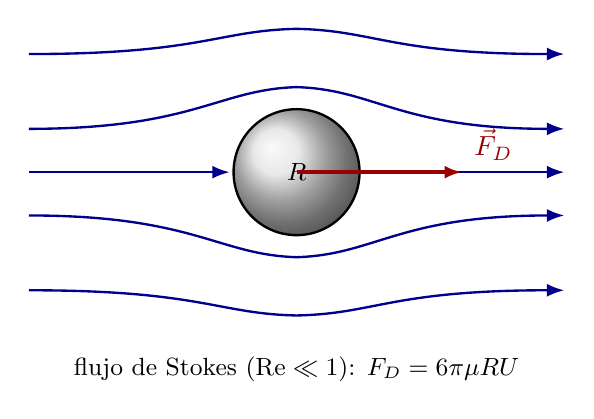
\begin{tikzpicture}[line width=0.85pt,>={Latex[length=2.2mm]}]
  \shade[ball color=black!12] (0,0) circle(0.8); \draw (0,0) circle(0.8);
  \node at (0,0){\small$R$};
  % lineas de corriente simetricas (reptante)
  \foreach \s in {1,-1}{
    \draw[blue!55!black,->] (-3.4,\s*0.55) .. controls (-1.3,\s*0.55) and (-1.0,\s*1.05) .. (0,\s*1.08) .. controls (1.0,\s*1.05) and (1.3,\s*0.55) .. (3.4,\s*0.55);
    \draw[blue!55!black,->] (-3.4,\s*1.5) .. controls (-1.2,\s*1.5) and (-1.0,\s*1.8) .. (0,\s*1.82) .. controls (1.0,\s*1.8) and (1.2,\s*1.5) .. (3.4,\s*1.5);}
  \draw[blue!55!black,->] (-3.4,0)--(-0.85,0); \draw[blue!55!black,->] (0.85,0)--(3.4,0);
  % arrastre
  \draw[->,red!60!black,line width=1.3pt] (0,0)--(2.1,0); \node[red!60!black] at (2.5,0.35){$\vec F_D$};
  \node at (0,-2.5){\small flujo de Stokes ($\mathrm{Re}\ll1$): $F_D=6\pi\mu R U$};
\end{tikzpicture}
\end{document}
